% !TEX root = Bachelorarbeit.tex
\subsection{The Take-Grant Model}	
Protection or acces control models specify, analyse and implemente security policies. 
The classical Take-Grant Model was primary introduced by Lipton and Snyder, 1977 in  \href{https://www.cs.nmt.edu/~doshin/t/s06/cs589/pub/2.JLS-TG.pdf}{%
"A Linear Time Algorithm for Deciding Subject Security"} \cite{1TG}.
\subsubsection{The Classical Model}
In the Take-Grant Model \cite{TakeG} subjects or objects are represented as nodes and authority as arcs in a directed graph that represents the system. \\ 
Rules for graph mutation represent the different system operations to modify  the authority distibution. 
The most common rules in the classical model are \textit{take, grant, create} and \textit{remove}. 
	
\begin{itemize}
\item \textbf{take rule}: Let S,X,Y be three distinct vertices in the protection graph with an arc, labelled with $\alpha$, from X to Y and one labelled with $\gamma$ from S to X, such that t $\in \gamma.$  
\begin{figure}[ht]
\centering
	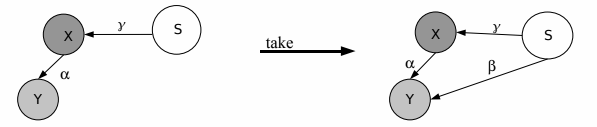
\includegraphics[width=0.7\textwidth]{./Pictures/takeRule.png}
	\caption[take rule]{\textit{Take} adds an edge from S to Y with the label $\beta \subseteq \alpha$. \cite{TakeG}}
	\label{fig:cltake}
\end{figure}	
	
\item \textbf{grant rule}:	Let S,X,Y agein be three distinct vertices in the graph with an arc, labelled with  $\alpha$, from S to Y and one labelled with $\gamma$ from S to X, such that g $\in \gamma$. 
\begin{figure}[ht]
\centering
	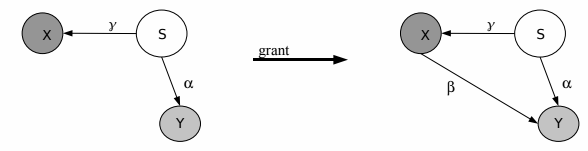
\includegraphics[width=0.7\textwidth]{./Pictures/grantRule.png}
	\caption[grant rule]{\textit{Grant} adds an edge from X to Y with the label $\beta \subseteq \alpha$.  \cite{TakeG}}
	\label{fig:clgrant}
\end{figure}	
	
\item \textbf{create rule}: Let S be a vertex in the graph. 
\begin{figure}[H]
\centering
	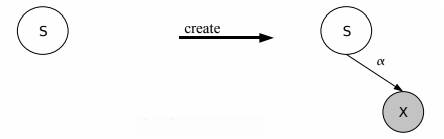
\includegraphics[width=0.5\textwidth]{./Pictures/createRule.png}
	\caption[create rule]{\textit{Create} adds a new node X and an arc from S to X, labelled with $\alpha$. \cite{TakeG}}
	\label{fig:clcreate}
\end{figure}	

\item \textbf{remove rule}: Let S, X be vertices in the graph with an arc from S to X, labelled with $\alpha$. 
\begin{figure}[H]
\centering
	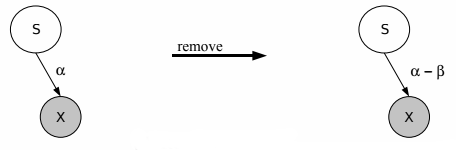
\includegraphics[width=0.5\textwidth]{./Pictures/removeRule.png}
	\caption[remove rule]{\textit{Remove} deletes $\beta$ labels from $\alpha$ or the arc itself if $\alpha - \beta = \lbrace\rbrace$. \cite{TakeG}}
	\label{fig:clremove}
\end{figure}		
\end{itemize}	
	
\subsubsection{Take-Grant specified for the seL4}\label{specT}
The Take-Grant Model specified in the paper "Verified Protection Model of the seL4 Microkernel" \cite{TakeG} is a variant of the classical Take-Grant model. \\
From the modifications made the one on the \textit{create rule} is the most important one. As I explained in chapter \ref{sec:seL4} authority in the kernel is implemented with capabilities. Adding a new node to the protection graph in the model corresponds to the creation of a new object with a capability pointing on it in the kernel. Therefore the object executing the \texttt{create operation} needs a capability with \texttt{create} authority. \\
The \textit{remove rule} was modified as it does not remove parts of labels anymore but the whole capability. That means the complete arc pointing on an object is removed. \\
To diminish authority a capability has to be removed and newly created with diminished authority. \\
With \texttt{retype} newly created capabilities are saved in a \textit{Capability Derivation Tree} (CDT) as children of the UMO. A capability can be copied with the \texttt{mint} or \texttt{imitate operation}. \\ 
A capability  copied with \texttt{mint} is inserted in the CDT as child of the original one. Those that are copied with \texttt{imitate} are siblings. Figure \ref{fig:cdt} showes a CDT where C1 and C2 are created from the UMO via \texttt{retype}. C3 and C4 are copied from C1 via \texttt{mint}. So they have the same or less authority as C1. C1' is copied from C1 via \texttt{imitate}. This operation transfers the same rights to the new capability. As a consequence the capability is inserted a sibling of C1. \\
	\begin{figure}[H]
	\centering
	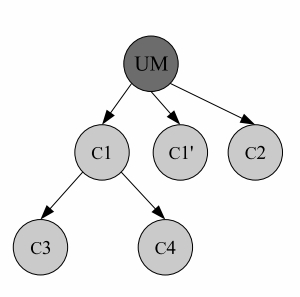
\includegraphics[width=0.3\textwidth]{./Pictures/CDT.jpg}
	\caption[CDT]{Example CDT with children and siblings \cite{PhDseL4}}
	\label{fig:cdt}
	\end{figure}
To remove a set of capabilities the operation \texttt{revoke} was implemented. \\ 
With this operation \texttt{remove} is executed on every capability that is in the CDT below the target capability. \\
A speciality of the extended model is, that objects and subjects are called \textit{entities}.\\
The goal of the paper "Verified Protection Model of the seL4 Microkernel" was to show that implementing isolated subsystems, using the mechanisms of the seL4 kernel, can be accomplished. \cite{TakeG} \\
Isolated subsystems are implemented as a collection of \textit{connected} entities. An entity that has \textit{grant authority} on another one is connected with this entity. Authority can neither get in nor get out of these isolated subsystems.\\
The exact specificaton of subsystems and entities follows in Chapter \ref{sec:Formalisation}.